\documentclass[11pt]{article}
\usepackage{graphicx}
\usepackage{url}
\usepackage[small]{caption}
\renewcommand{\baselinestretch}{1.0}
\title{Project 2 - Evolving Izhikevich neurons}
\author{Knut Halvor Skrede}
\setlength{\parindent}{0pt}
\setlength{\parskip}{2ex} 
\begin{document}
\maketitle

\section*{1 System description}

\subsection*{Genotype representation}

The genotype is represented as a boolean array of size $5*20$. 20 bits represent each of the
5 variables to evolve.

\subsection*{Phenotype representation}

The phenotype is represented as a integer array of size 5. Each integer represent one of the
parameters for the Izhikevich function. Since the genotype is represented as a boolean array of
size $5*20$, each of the 5 parameters can hold $2^{20}$ different values within their range.

$A \in [0.001, 0.2]$ $B \in [0.01, 0.3]$ $C \in [−80, −30]$ $D \in [0.1, 10]$ $K \in [0.01, 1.0]$

These values are then used to create the spike train as proposed by section 2 of the assignment.

Initializing the variables

$v = -60$\\
$u = 0$\\

Calculating the derivatives

$v' = \frac{1}{\tau}*(k*v^2 + 5*v +140 - u -I)$\\
$u' = \frac{a}{\tau}*(b*v - u)$\\

Updating v and u

$v = v+v'$\\
$u = u+u'$\\

Storing v as the value in the spiketrain.

Resetting v and u when they exceed the threshold

$v = c$\\
$u = u+d$\\

By repeating this N times, the spiketrain has been created.

\subsection*{Fitness evaluation}

The fitness evaluation is based on the three main distance metrics proposed by the project
description. Spike time distance metric, Spike interval distance metric and the Waveform
distance metric. In addition, a spike-count difference penalty is added to each of these
evaluation routines. Since the objektive is to minimize the distances, the fitness evaluation
returns the inverse of the chosen distance metric.

\section*{2 Test cases}

\begin{figure}
\begin{center}
\mbox{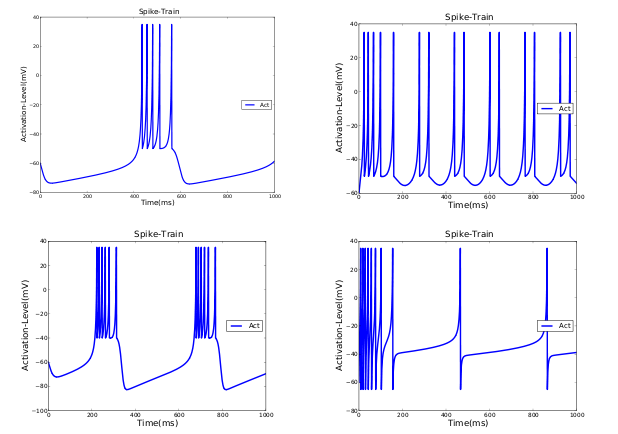
\includegraphics[width=0.99\textwidth]{images/ref.png}}
\end{center}
\caption{Plots copied from the assignment, included as reference.}
\label{fig:0}
\end{figure}

I have only included the best found results for each test case. See figure \ref{fig:0} to compare to
target spike trains from assignment.

\subsection*{1 - Input 1, Spike time distance metric}

\begin{figure}
\begin{center}
\mbox{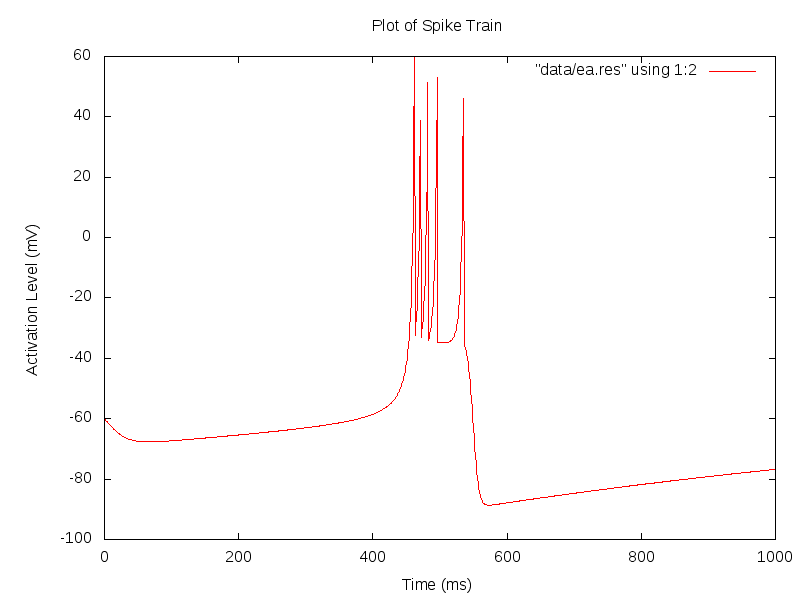
\includegraphics[width=0.49\textwidth]{images/1-res.png}}
\mbox{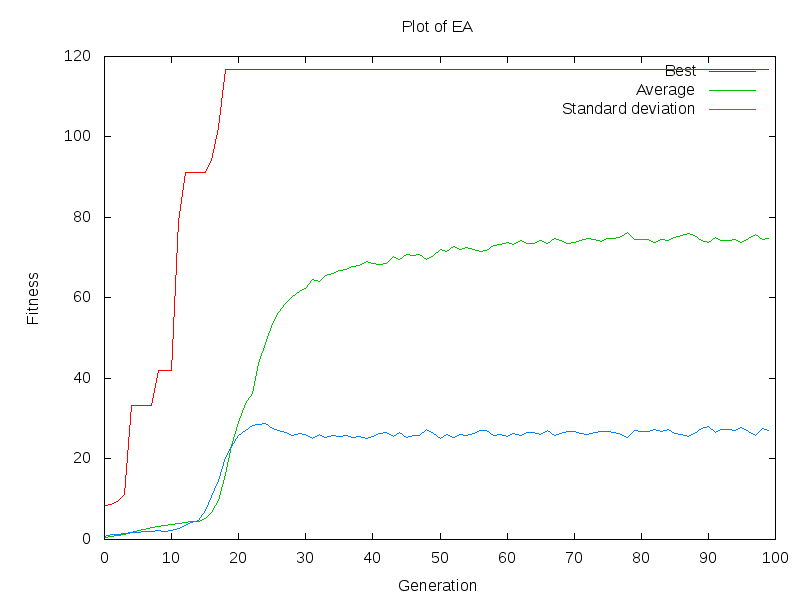
\includegraphics[width=0.49\textwidth]{images/1-fit.png}}
\end{center}
\caption{Left: Plot of the Izhikevich model with the evolved parameters\\
Right: Fitness plot of the evolutionary run resulting in the parameters.}
\label{fig:1}
\end{figure}

Settings used for the EA:

1: Size of child pool: 2000\\
2: Size of adult pool: 2000\\
3: number of generations: 100\\
4: mutation rate: 0.1\\
5: crossover rate: 0.85\\
6: selection protocol: Full generational replacement\\
7: selection strategy: Fitness proportionate\\
8: elitism: 1\\

Resulting parameters:

A=0.0212307 B=0.0868231 C=-34.6432 D=7.62903 K=0.0409677

See figure \ref{fig:1} for plots.

\subsection*{2 - Input 1, Spike interval distance metric}

\begin{figure}
\begin{center}
\mbox{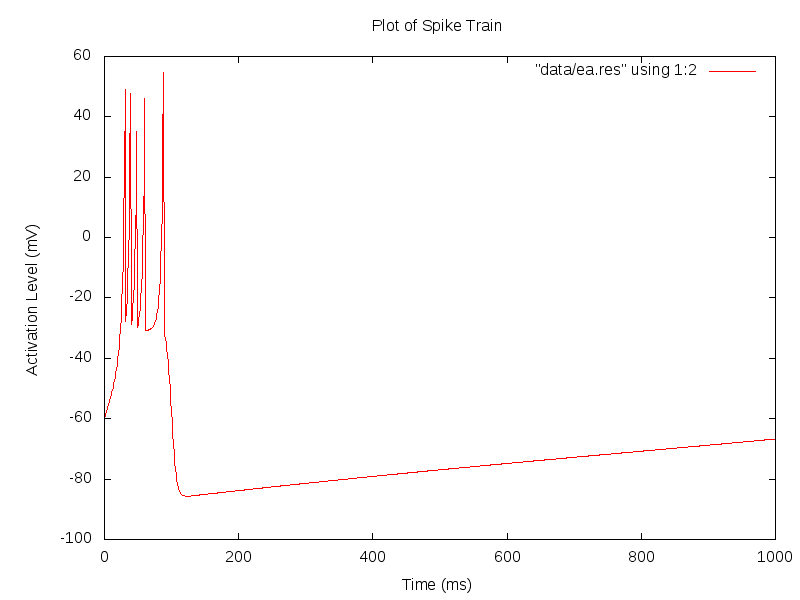
\includegraphics[width=0.49\textwidth]{images/2-res.png}}
\mbox{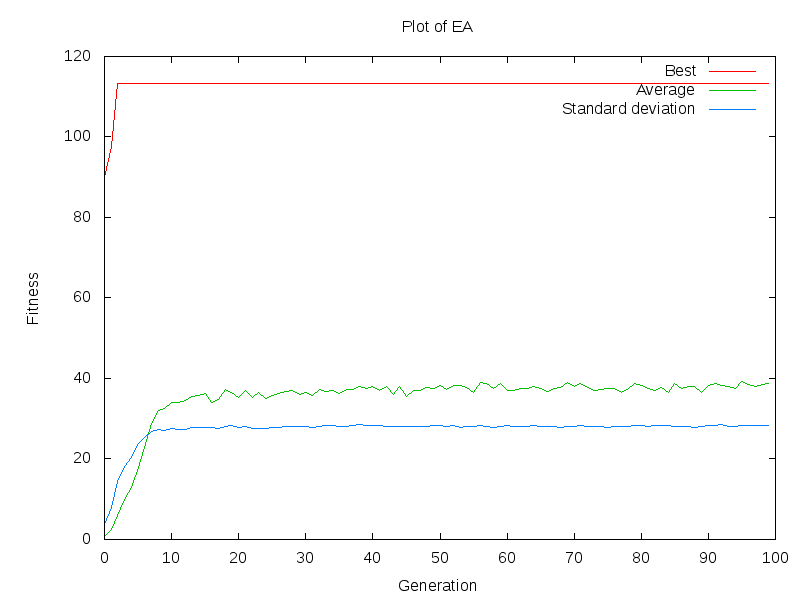
\includegraphics[width=0.49\textwidth]{images/2-fit.png}}
\end{center}
\caption{Left: Plot of the Izhikevich model with the evolved parameters\\
Right: Fitness plot of the evolutionary run resulting in the parameters.}
\label{fig:2}
\end{figure}

Settings used for the EA:

1: Size of child pool: 2000\\
2: Size of adult pool: 2000\\
3: number of generations: 100\\
4: mutation rate: 0.8\\
5: crossover rate: 0.85\\
6: selection protocol: Full generational replacement\\
7: selection strategy: Fitness proportionate\\
8: elitism: 1\\

Resulting parameters:

A=0.0144223 B=0.0153861 C=-30.7331 D=9.65161 K=0.043871

The spike interval distance metric consistently found solutions
that where shifted to the left of the target spiketrain.

See figure \ref{fig:2} for plots.

\subsection*{3 - Input 1, Waveform distance metric}

\begin{figure}
\begin{center}
\mbox{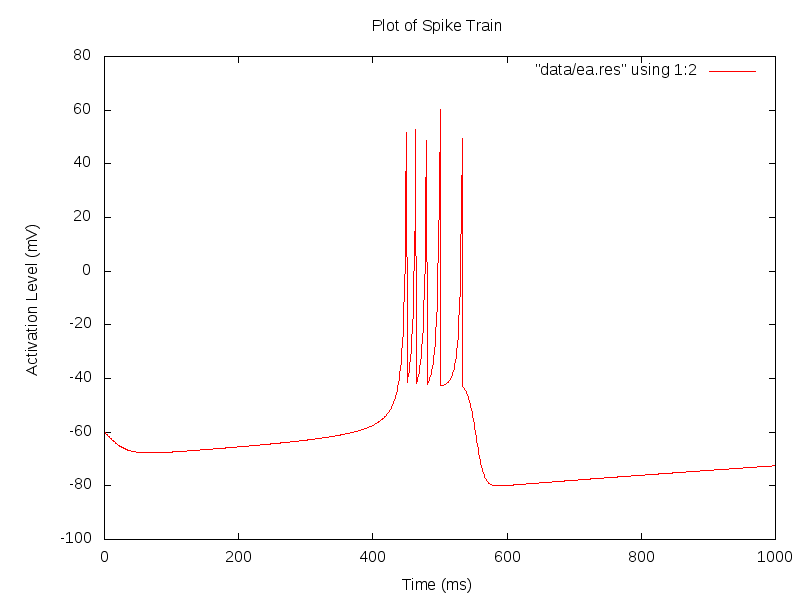
\includegraphics[width=0.49\textwidth]{images/3-res.png}}
\mbox{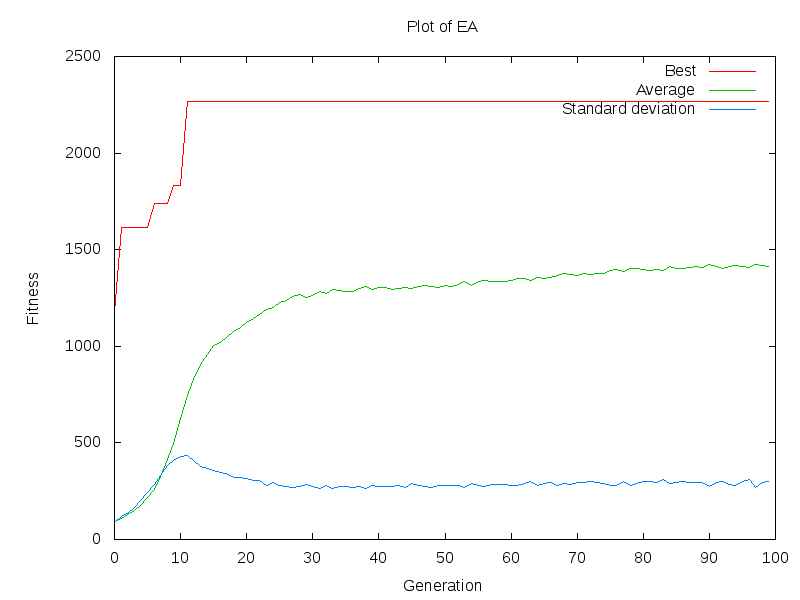
\includegraphics[width=0.49\textwidth]{images/3-fit.png}}
\end{center}
\caption{Left: Plot of the Izhikevich model with the evolved parameters\\
Right: Fitness plot of the evolutionary run resulting in the parameters.}
\label{fig:3}
\end{figure}

Settings used for the EA:

1: Size of child pool: 2000\\
2: Size of adult pool: 2000\\
3: number of generations: 100\\
4: mutation rate: 0.2\\
5: crossover rate: 0.85\\
6: selection protocol: Full generational replacement\\
7: selection strategy: Sigma scaling\\
8: elitism: 1\\

Resulting parameters:

A=0.0146168 B=0.116305 C=-42.7077 D=3.7 K=0.0409677

See figure \ref{fig:3} for plots.

\subsection*{4 - Input 2, Spike timel distance metric}

\begin{figure}
\begin{center}
\mbox{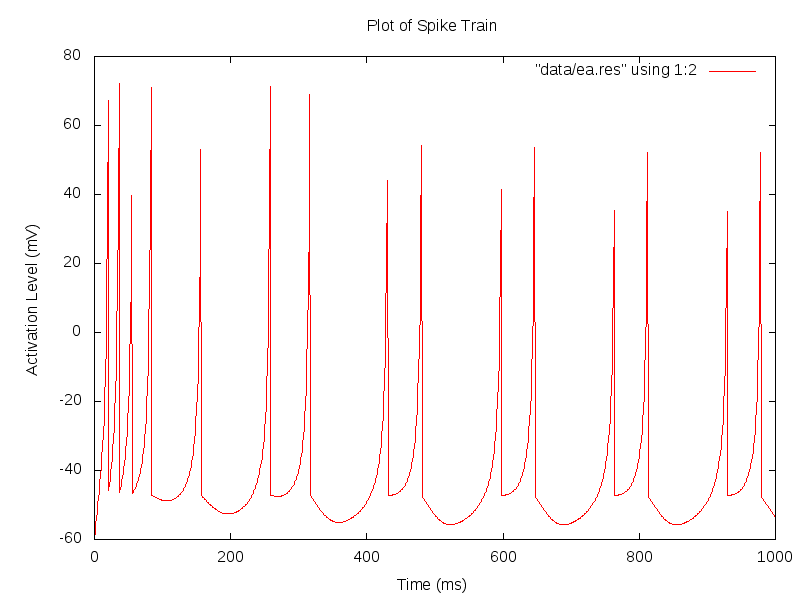
\includegraphics[width=0.49\textwidth]{images/4-res.png}}
\mbox{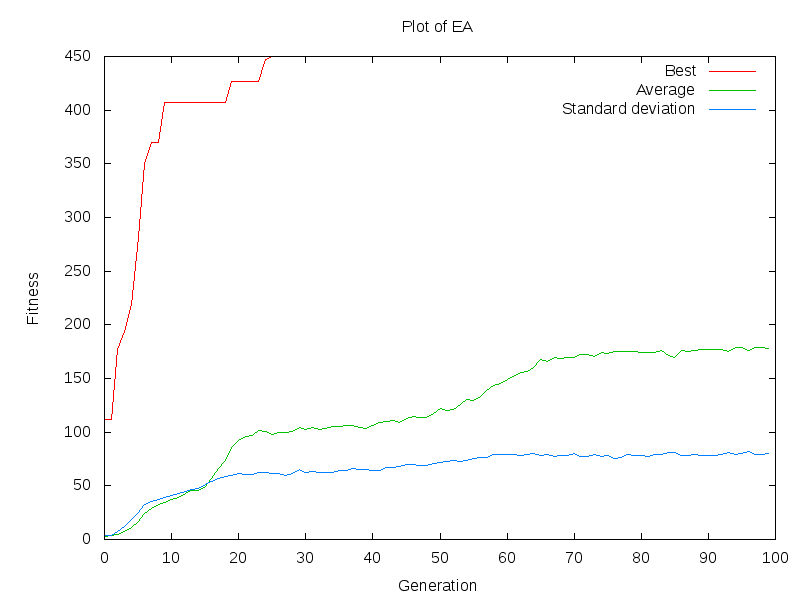
\includegraphics[width=0.49\textwidth]{images/4-fit.png}}
\end{center}
\caption{Left: Plot of the Izhikevich model with the evolved parameters\\
Right: Fitness plot of the evolutionary run resulting in the parameters.}
\label{fig:4}
\end{figure}

Settings used for the EA:

1: Size of child pool: 2000\\
2: Size of adult pool: 2000\\
3: number of generations: 100\\
4: mutation rate: 0.2\\
5: crossover rate: 0.85\\
6: selection protocol: Full generational replacement\\
7: selection strategy: Fitness proportionate\\
8: elitism: 1\\

Resulting parameters:

A=0.0292063 B=0.156559 C=-47.1065 D=6.23548 K=0.0477419

See figure \ref{fig:4} for plots.

\subsection*{5 - Input 2, Spike interval distance metric}

\begin{figure}
\begin{center}
\mbox{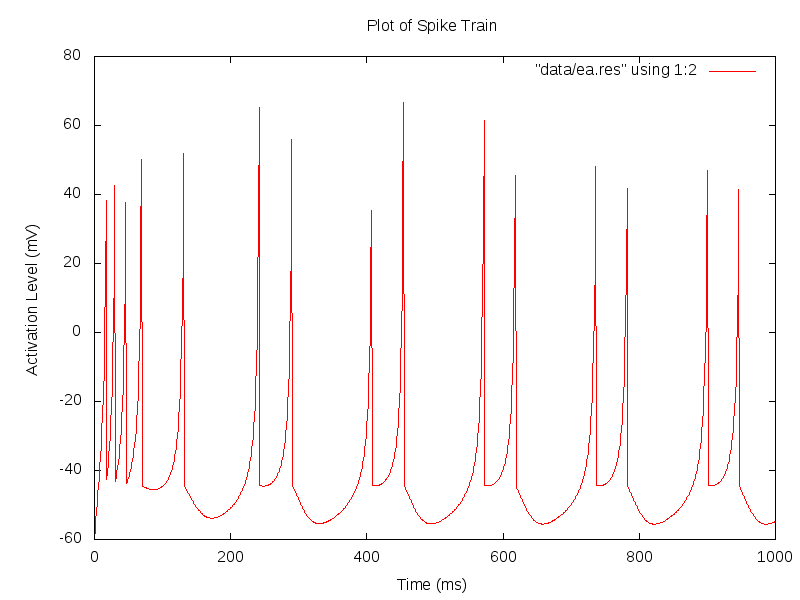
\includegraphics[width=0.49\textwidth]{images/5-res.png}}
\mbox{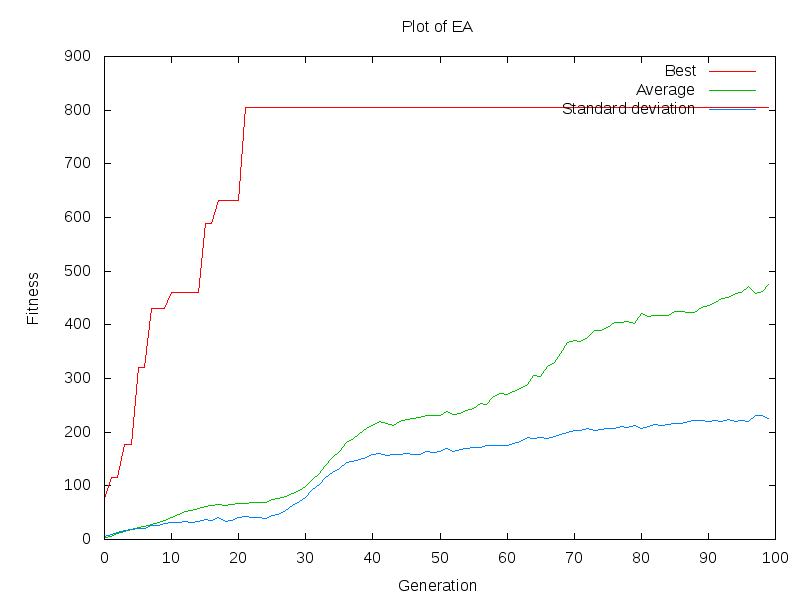
\includegraphics[width=0.49\textwidth]{images/5-fit.png}}
\end{center}
\caption{Left: Plot of the Izhikevich model with the evolved parameters\\
Right: Fitness plot of the evolutionary run resulting in the parameters.}
\label{fig:5}
\end{figure}

Settings used for the EA:

1: Size of child pool: 2000\\
2: Size of adult pool: 2000\\
3: number of generations: 100\\
4: mutation rate: 0.2\\
5: crossover rate: 0.85\\
6: selection protocol: Full generational replacement\\
7: selection strategy: Fitness proportionate\\
8: elitism: 1\\

Resulting parameters:

A=0.0294008 B=0.169599 C=-44.3695 D=7.59032 K=0.0496774

See figure \ref{fig:5} for plots.

\subsection*{6 - Input 2, Waveform distance metric}

\begin{figure}
\begin{center}
\mbox{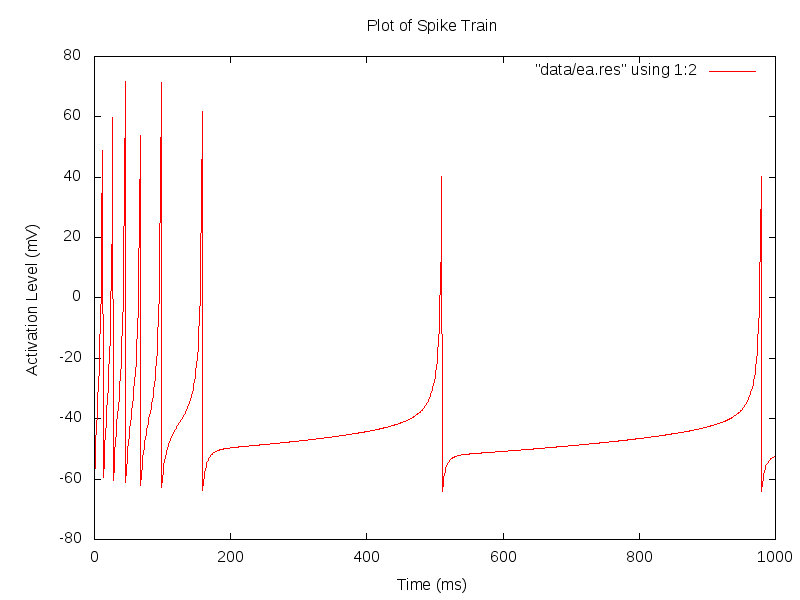
\includegraphics[width=0.49\textwidth]{images/6-res.png}}
\mbox{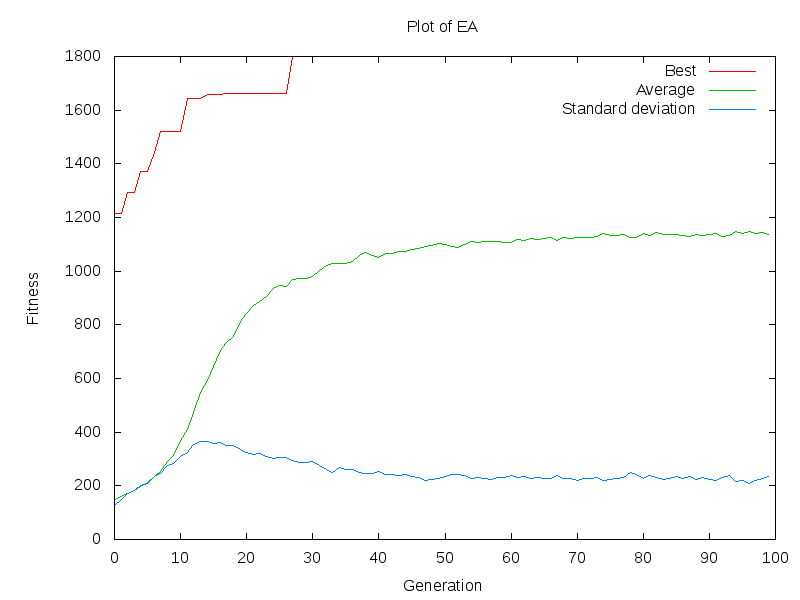
\includegraphics[width=0.49\textwidth]{images/6-fit.png}}
\end{center}
\caption{Left: Plot of the Izhikevich model with the evolved parameters\\
Right: Fitness plot of the evolutionary run resulting in the parameters.}
\label{fig:6}
\end{figure}

Settings used for the EA:

1: Size of child pool: 2000\\
2: Size of adult pool: 2000\\
3: number of generations: 100\\
4: mutation rate: 0.2\\
5: crossover rate: 0.85\\
6: selection protocol: Full generational replacement\\
7: selection strategy: Boltzmann selection\\
8: elitism: 1\\
9: Temperature: 1000\\

Resulting parameters:

A=0.00352884 B=0.0941936 C=-67.2923 D=8.8 K=0.0603226

See figure \ref{fig:6} for plots.

\subsection*{7 - Input 3, Spike time distance metric}

\begin{figure}
\begin{center}
\mbox{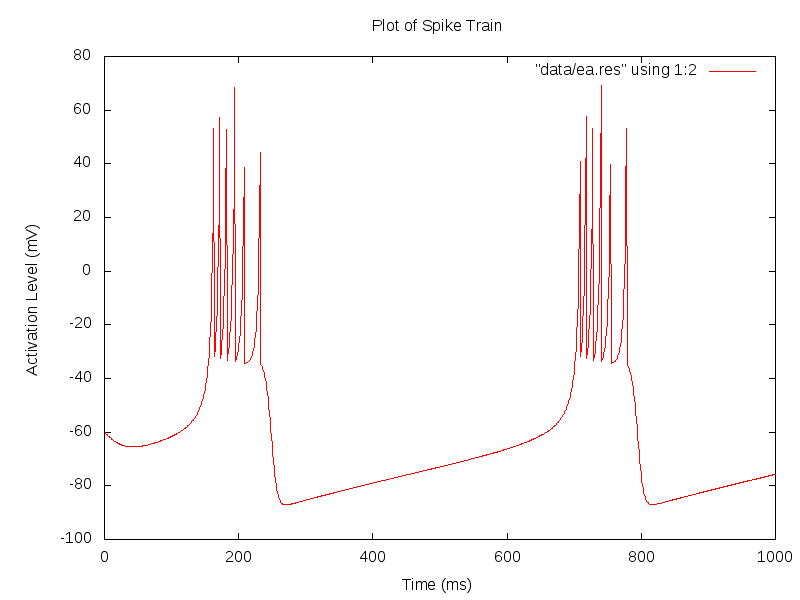
\includegraphics[width=0.49\textwidth]{images/7-res.png}}
\mbox{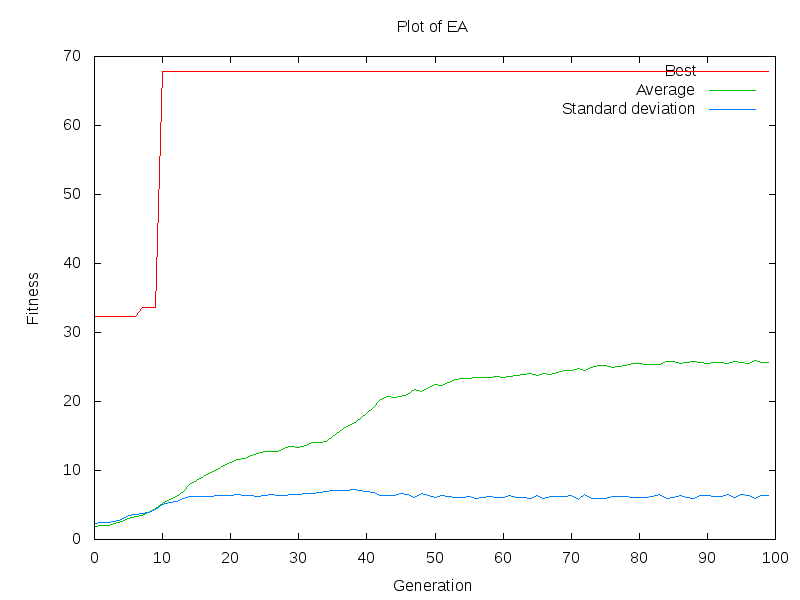
\includegraphics[width=0.49\textwidth]{images/7-fit.png}}
\end{center}
\caption{Left: Plot of the Izhikevich model with the evolved parameters\\
Right: Fitness plot of the evolutionary run resulting in the parameters.}
\label{fig:7}
\end{figure}

Settings used for the EA:

1: Size of child pool: 2000\\
2: Size of adult pool: 2000\\
3: number of generations: 100\\
4: mutation rate: 0.2\\
5: crossover rate: 0.85\\
6: selection protocol: Full generational replacement\\
7: selection strategy: Sigma scaling\\
8: elitism: 1\\

Resulting parameters:

A=0.0344585 B=0.201916 C=-34.35 D=6.73871 K=0.0409677

See figure \ref{fig:7} for plots.

\subsection*{8 - Input 3, Spike interval distance metric}

Settings used for the EA:

1: Size of child pool: 2000\\
2: Size of adult pool: 2000\\
3: number of generations: 100\\
4: mutation rate: 0.2\\
5: crossover rate: 0.85\\
6: selection protocol: Full generational replacement\\
7: selection strategy: Sigma scaling\\
8: elitism: 1\\

Resulting parameters:

A=0.0329022 B=0.140401 C=-36.4516 D=5.27742 K=0.0419355

See figure \ref{fig:8} for plots.

\begin{figure}
\begin{center}
\mbox{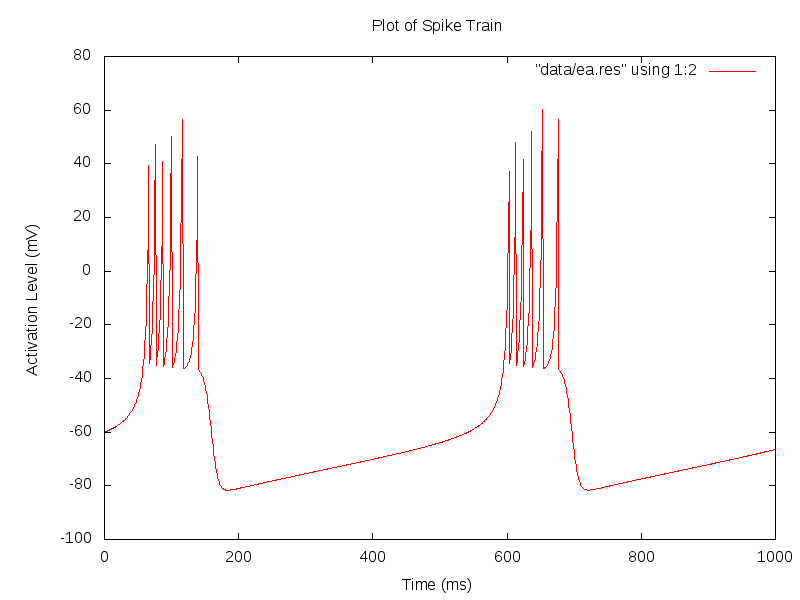
\includegraphics[width=0.49\textwidth]{images/8-res.png}}
\mbox{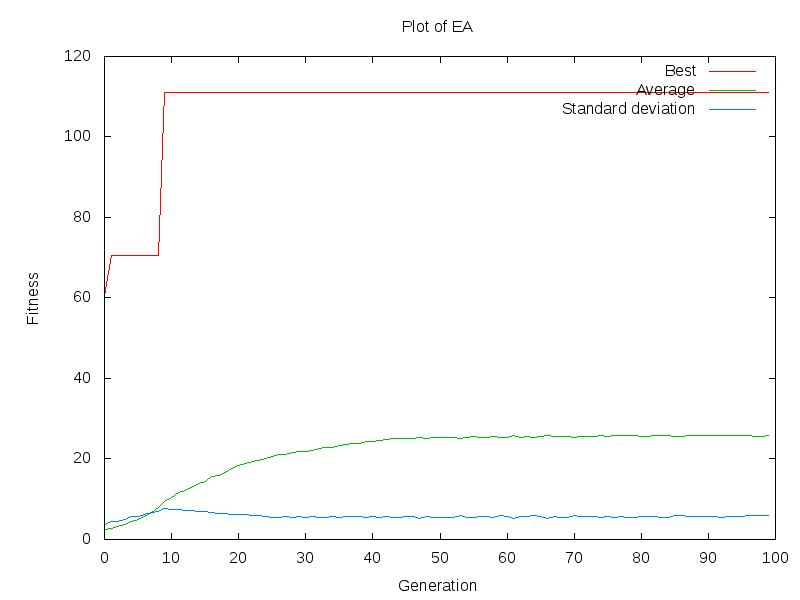
\includegraphics[width=0.49\textwidth]{images/8-fit.png}}
\end{center}
\caption{Left: Plot of the Izhikevich model with the evolved parameters\\
Right: Fitness plot of the evolutionary run resulting in the parameters.}
\label{fig:8}
\end{figure}



\subsection*{9 - Input 3, Waveform distance metric}

Settings used for the EA:

1: Size of child pool: 2000\\
2: Size of adult pool: 2000\\
3: number of generations: 100\\
4: mutation rate: 0.2\\
5: crossover rate: 0.85\\
6: selection protocol: Full generational replacement\\
7: selection strategy: Sigma scaling\\
8: elitism: 1\\

Resulting parameters:

A=0.124524 B=0.0604594 C=-37.6735 D=6.96129 K=0.0409677

See figure \ref{fig:9} for plots.

\begin{figure}
\begin{center}
\mbox{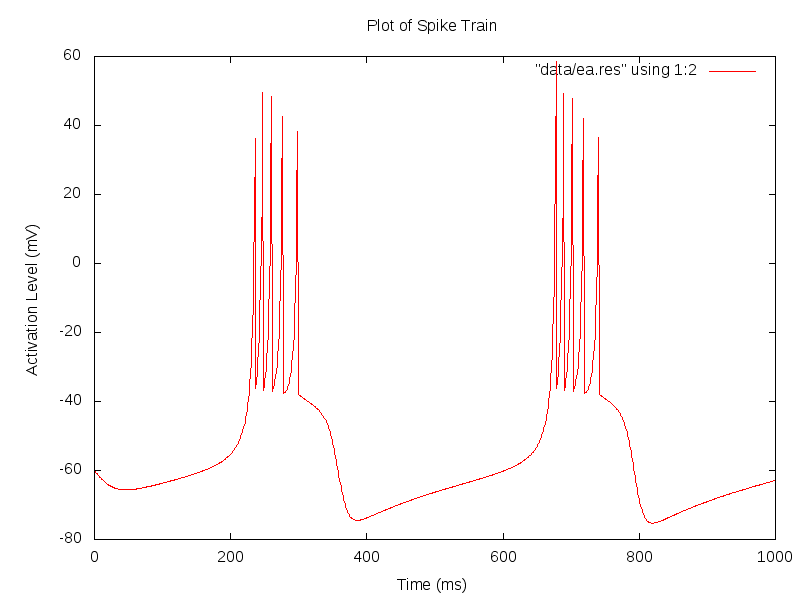
\includegraphics[width=0.49\textwidth]{images/9-res.png}}
\mbox{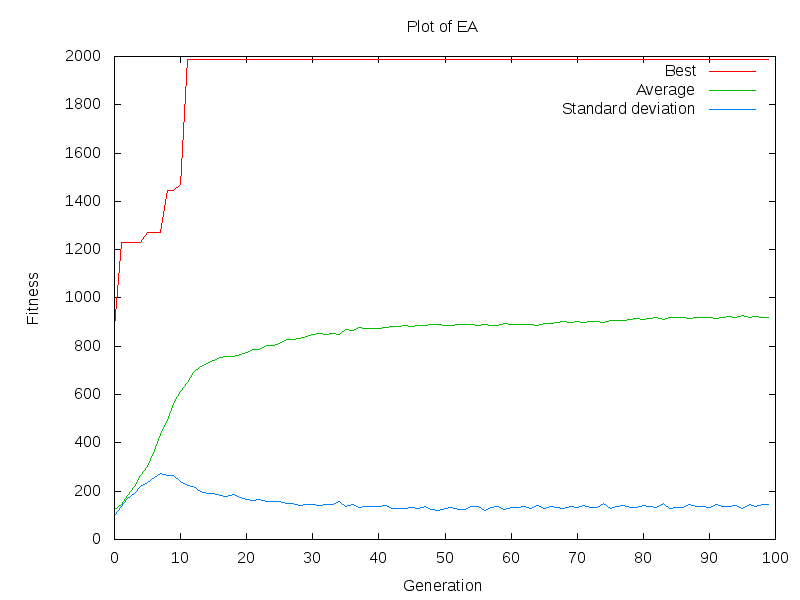
\includegraphics[width=0.49\textwidth]{images/9-fit.png}}
\end{center}
\caption{Left: Plot of the Izhikevich model with the evolved parameters\\
Right: Fitness plot of the evolutionary run resulting in the parameters.}
\label{fig:9}
\end{figure}


\subsection*{10 - Input 4, Spike time distance metric}

Settings used for the EA:

1: Size of child pool: 2000\\
2: Size of adult pool: 2000\\
3: number of generations: 100\\
4: mutation rate: 0.2\\
5: crossover rate: 0.85\\
6: selection protocol: Full generational replacement\\
7: selection strategy: Sigma scaling\\
8: elitism: 1\\

Resulting parameters:

A=0.00313979 B=0.104399 C=-46.9599 D=8.57742 K=0.0709677

See figure \ref{fig:10} for plots.

\begin{figure}
\begin{center}
\mbox{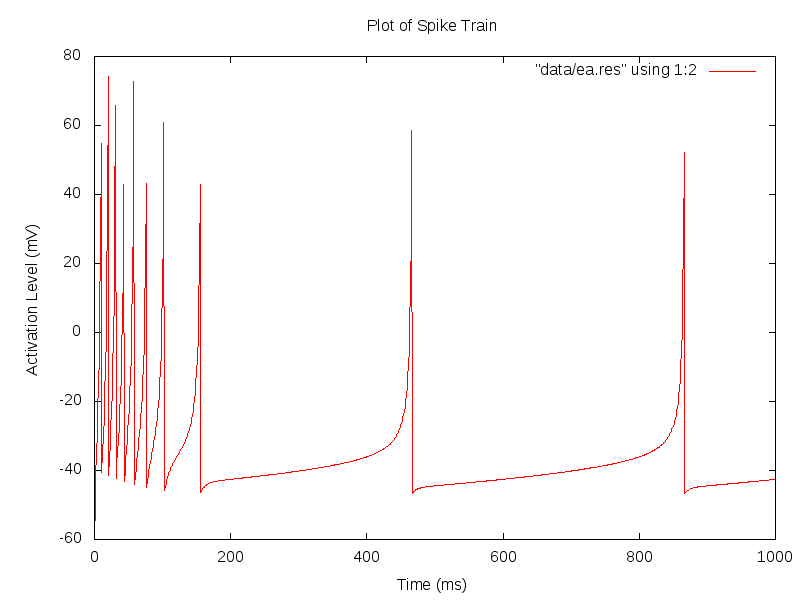
\includegraphics[width=0.49\textwidth]{images/10-res.png}}
\mbox{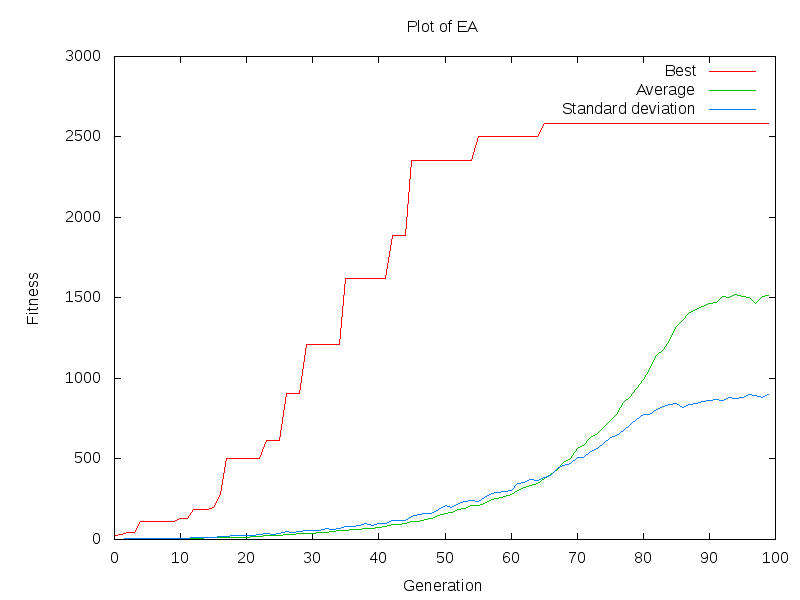
\includegraphics[width=0.49\textwidth]{images/10-fit.png}}
\end{center}
\caption{Left: Plot of the Izhikevich model with the evolved parameters\\
Right: Fitness plot of the evolutionary run resulting in the parameters.}
\label{fig:10}
\end{figure}

\subsection*{11 - Input 4, Spike interval distance metric}

This run gained a fitness of 100 000, this is the value the fitness is set to
if the SDM calculate a distance of 0 or 0.01.

Settings used for the EA:

1: Size of child pool: 2000\\
2: Size of adult pool: 2000\\
3: number of generations: 100\\
4: mutation rate: 0.2\\
5: crossover rate: 0.85\\
6: selection protocol: Full generational replacement\\
7: selection strategy: Sigma scaling\\
8: elitism: 1\\

Resulting parameters:

A=0.00294526 B=0.282141 C=-60.2542 D=9.81613 K=0.0787097

See figure \ref{fig:11} for plots.

\begin{figure}
\begin{center}
\mbox{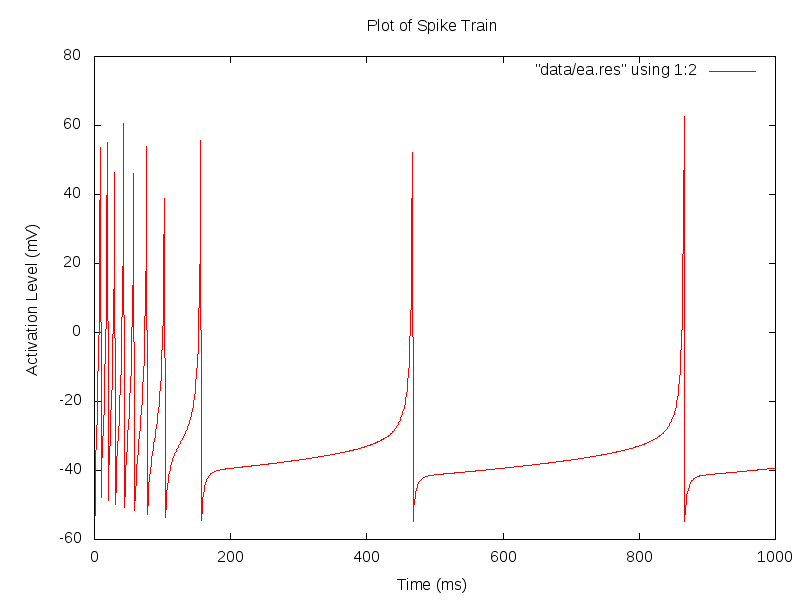
\includegraphics[width=0.49\textwidth]{images/11-res.png}}
\mbox{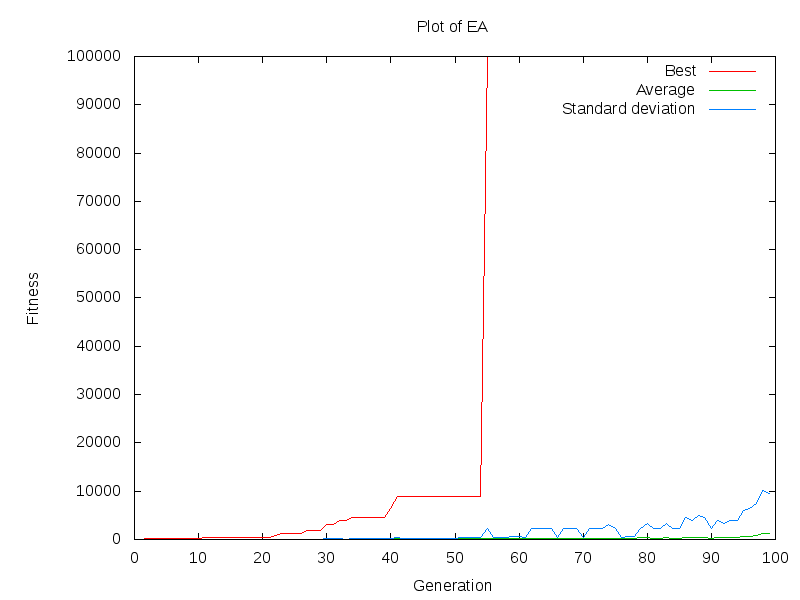
\includegraphics[width=0.49\textwidth]{images/11-fit.png}}
\end{center}
\caption{Left: Plot of the Izhikevich model with the evolved parameters\\
Right: Fitness plot of the evolutionary run resulting in the parameters.}
\label{fig:11}
\end{figure}



\subsection*{12 - Input 4, Waveform distance metric}

\begin{figure}
\begin{center}
\mbox{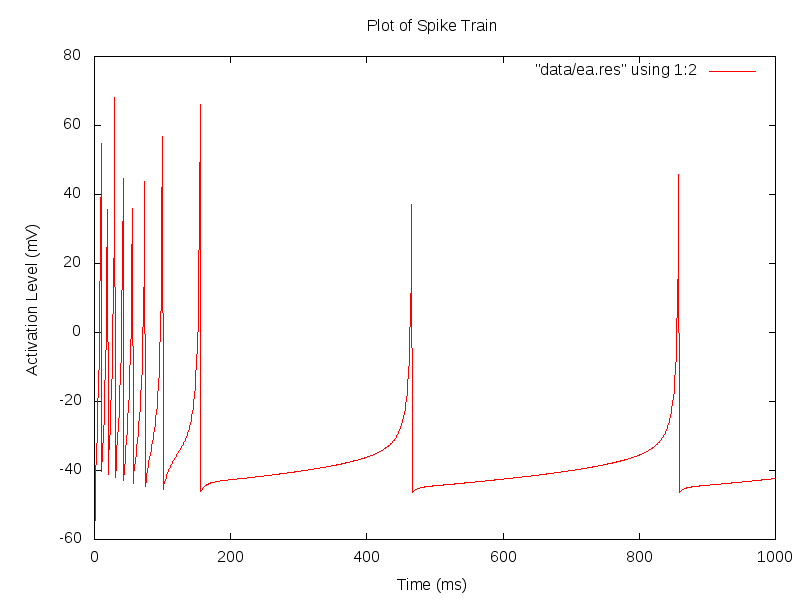
\includegraphics[width=0.49\textwidth]{images/12-res.png}}
\mbox{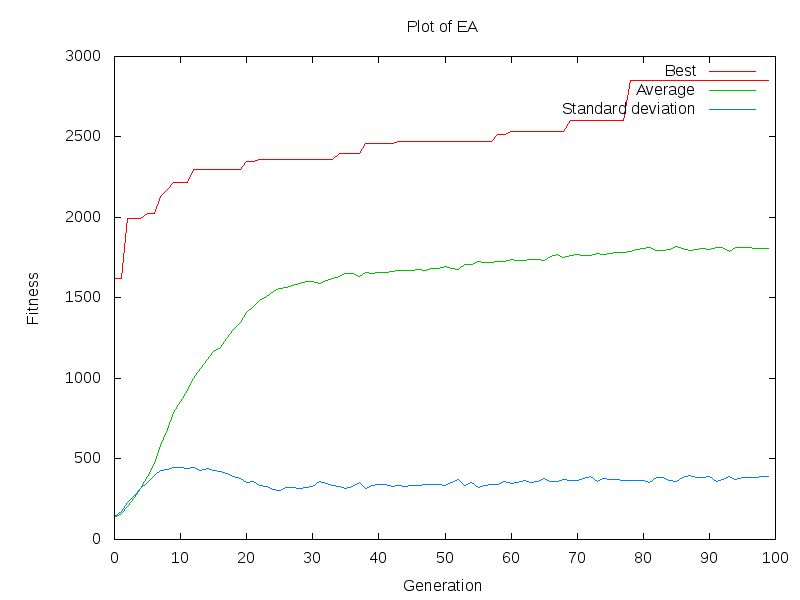
\includegraphics[width=0.49\textwidth]{images/12-fit.png}}
\end{center}
\caption{Left: Plot of the Izhikevich model with the evolved parameters\\
Right: Fitness plot of the evolutionary run resulting in the parameters.}
\label{fig:12}
\end{figure}

Settings used for the EA:

1: Size of child pool: 2000\\
2: Size of adult pool: 2000\\
3: number of generations: 100\\
4: mutation rate: 0.2\\
5: crossover rate: 0.85\\
6: selection protocol: Full generational replacement\\
7: selection strategy: Sigma scaling\\
8: elitism: 1\\

Resulting parameters:

A=0.00333431 B=0.0443011 C=-46.6178 D=8.60645 K=0.0709677

See figure \ref{fig:12} for plots.

\section*{3 Genotype - phenotype mapping classification}

What we are evolving here is the parameters for the spike train. The creation of the spike train itself
could be said to be part of the developmental process, or the fitness evaluation. The genotype-phenotype
here is a simple boolean to floating point mapping, where the boolean genotype represent the discrete values possible
in the parameters range.

\section*{4 Practical implimactions}

The tool could be used to find the Izhikevich function that mimics an actual neuron. By doing an analysis
like this on multiple neurons (or a neural network), one could simulate these in an attempt to figure out
what is going on.

\section*{5 Other problem domains}

This method could be used for any problem that involves a fixed set of parameters to be found. However,
a method of fitness evaluation must exist for the problem.

A more similar problem, where the implemented SDM's could be used, would be curve fitting.
Parameters for any function could be evolved in an attempt to minimize the distance to some test data.

\end{document}


